\documentclass[tikz]{standalone}
\usetikzlibrary{arrows.meta,angles}
\begin{document}
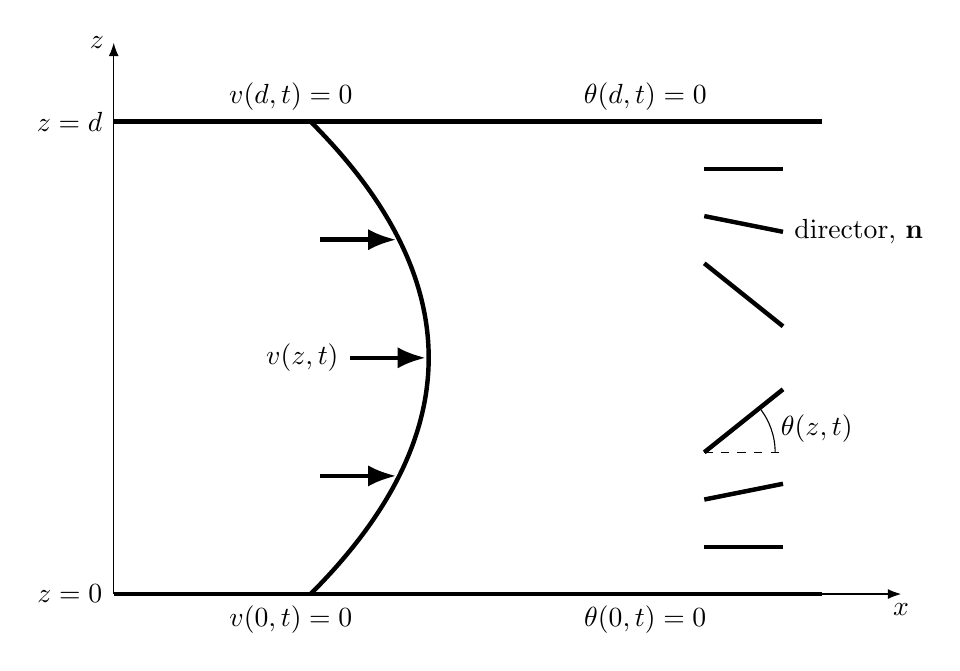
\begin{tikzpicture}[>=Latex, declare function={w=10; h=7;}]
% 1. Axis
\path[->] (0,0) edge node[at end, below]{$x$}  (w, 0) 
                edge node[at end, left]{$z$}   (0, h);
                
% 2. horizontal lines
\tikzset{every path/.append style=ultra thick}
\path (0,0) node[left]{$z=0$} edge[below] node[near start]{$v(0,t)=0$}
                                          node[near end]  {$\theta(0,t) = 0$}  (w - 1, 0)
   (0, h-1) node[left]{$z=d$} edge[above] node[near start]{$v(d,t)=0$}
                                          node[near end]  {$\theta(d,t) = 0$} +(w - 1, 0);
% 3. Arc
\draw (w/4, 0) .. controls (w/4+2, {(h-1)/2-1}) and (w/4+2, {(h-1)/2+1}).. +(0, h-1)
  foreach \pos[count=\i] in {near start, midway, near end}{
   % 3.1. and those arrows
   coordinate[\pos] (c-\i) (c-\i) edge[shorten <=1pt, <-] coordinate[at end] (cc-\i) ++ (left:1)
  }
  % 3.2. and that one node
  node[left] at (cc-2) {$v(z,t)$};

% 4. some weird lines
\foreach \y/\h[count=\i] in {.1/0 , .2/.2 , .3/.8 , .7/-.8 , .8/-.2, .9/0}
  \draw (3/4*w, {\y*(h-1)}) -- +(1, \h)
    coordinate[at start] (d-\i)
    coordinate[at end]   (e-\i);

% 4.1. with one text
\node[right] at (e-5) {director, \textbf{n}};

% 4.2. and that angle marking
\tikzset{every path/.append style=thin}
\draw[dashed] (d-3) -- +(right:1) coordinate (de-3);
\pic[draw, angle radius=.9cm, angle eccentricity=1,
     pic text options=right,pic text={$\theta(z, t)$}] {angle=de-3--d-3--e-3};
\end{tikzpicture}
\end{document}
